\documentclass[
  11pt,
  letterpaper,
   addpoints,
   %answers
  ]{exam}

\usepackage{../exercise-preamble}

\begin{document}

\noindent
\begin{minipage}{0.47\textwidth}

\includegraphics[width=\textwidth]{../fcfm_die}
\end{minipage}
\begin{minipage}{0.53\textwidth}
\begin{center} 
\large\textbf{Electromagnetismo Aplicado} (EL3103-1) \\
\large\textbf{Ejercicio 1} \\
\normalsize Prof.~Benjamin Jacard H.\\
\normalsize Prof.~Aux.~Erik Saez A.
\end{center}
\end{minipage}

\vspace{0.5cm}
\noindent
\vspace{.85cm}

\begin{questions}
    %%%%%%%%%%%%%%%%%%%%%%%%%%%%
    \question     
  
Una gran plancha de bronce de espesor \( \delta \) y conductividad \( \sigma \), tiene una corriente continua en la dirección \( x \) que produce un potencial \( \Phi = -E_0 x \). 
Considere ahora que se perfora un orificio de radio \( a \) a través de la plancha en el punto \( x = 0, y = 0 \).

\begin{itemize}
    \item[a)] Determine el potencial \( \Phi (r,\theta) \) en cualquier punto de los medios \( 1 \) y \( 2 \).
    \item[b)] ¿Cuál es la densidad de corriente \( \vec{J} \) resultante en cualquier punto del bronce? ¿Dónde ocurre y qué valor tiene la densidad de corriente máxima?
\end{itemize}

Nota: En coordenadas cilíndricas \( (r, \theta, z) \), una solución general de la ecuación \( \nabla^2 \Phi = 0 \), independiente de \( z \) y dependiente de \( \cos\theta \), está dada por:
\begin{equation}
    \Phi (r, \theta) = (Ar + \frac{B}{r}) \cos\theta
\end{equation}
Donde el gradiente es:
\begin{align}
    \nabla \Phi = \frac{\partial \Phi}{\partial r} \hat{r} + \frac{1}{r} \frac{\partial \Phi}{\partial \theta} \hat{\theta}
\end{align}
\begin{center}
    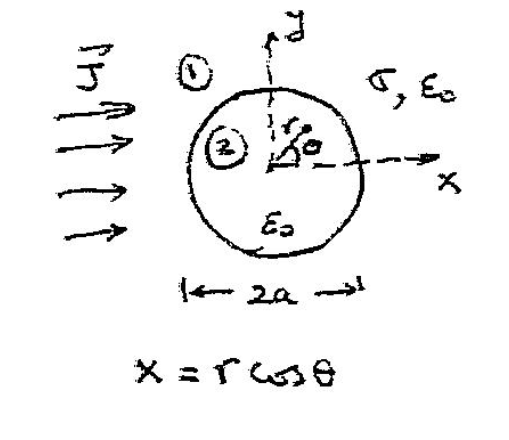
\includegraphics[width=0.4\textwidth]{Ejercicio_1_1}
    \captionof{figure}{Esquema del problema}
\end{center}
    %%%%%%%%%%%%%%%%%%%%%%%%%%%%
    \begin{solution}
        a
    \end{solution}
    %%%%%%%%%%%%%%%%%%%%%%%%%%%
    \newpage
    \question  
    Considere una línea coaxial infinitamente larga, en cuyo conductor de radio \( a \) la corriente total es \( I_0 \) y en el conductor exterior de radio \( b \) es \( -I_0 \).
    \begin{itemize}
        \item[i)] Determinar el campo magnético \( \vec{H} (r,\theta) \) en el dieléctrico (\( a < r < b \)).
        \item[ii)] Determinar la inductancia \( L \) de la línea por unidad de longitud según \( z \), en base a la energía almacenada en el campo magnético en el dieléctrico.
        \item[iii)] Determinar la inductancia \( L \) en base al flujo magnético en el dieléctrico.
    \end{itemize}
    \begin{center}
        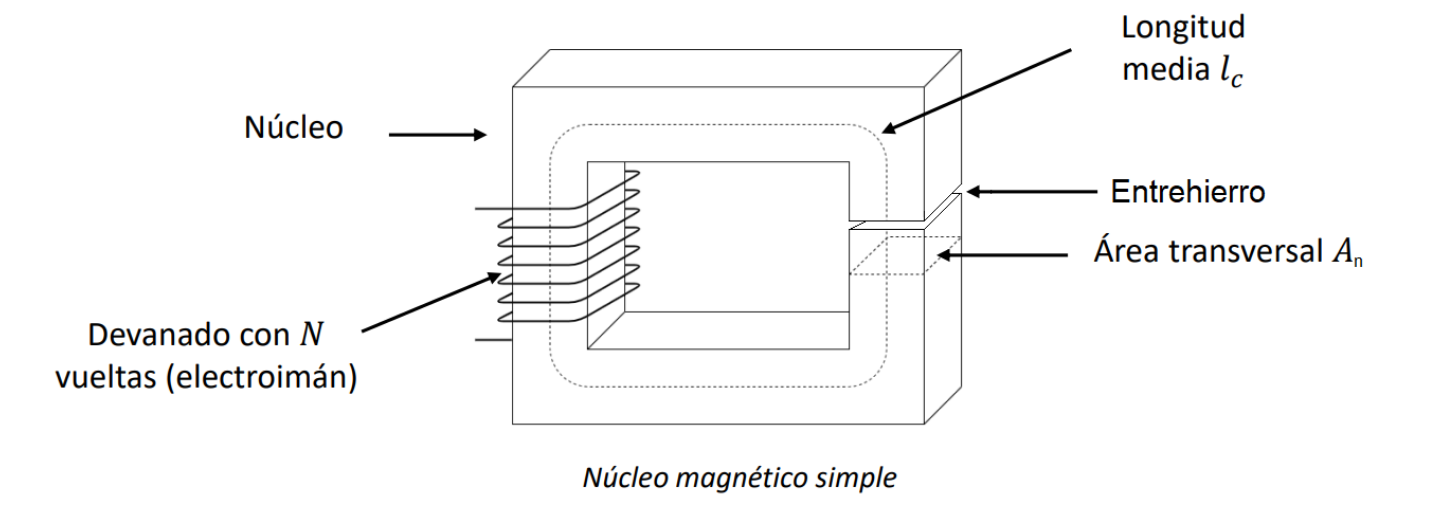
\includegraphics[width=0.3\textwidth]{Ejercicio_1_2}
        \captionof{figure}{Esquema del problema}
    \end{center}
    %%%%%%%%%%%%%%%%%%%%%%%%%%%
    \begin{solution}
        \begin{enumerate}
            \item Se dice que la geométrica corresponde a una estructura coaxial y por tanto será conveniente el utilizar coordenadas cilindricas.En relacion al enunciado,entre los medios notamos que no existe presencia de carga libre esto implicará que el Laplaciano sea $\sigma_f = 0$.Esto es posible derivarlo de Gauss en presencia de medios (Es importante esta consideracion, dado que la carga ligada esta presente en el desplazamiento y en el parametro $\epsilon$) en su forma  diferencial, es decir:
            \begin{equation}
                \Vec{\nabla} \cdot \textbf{E} = \frac{\rho_f}{\epsilon} 
            \end{equation}
            Se puede interpretar del hecho que cargas puntuales generan zonas de divergencia tanto positivas o negativas alrededor de ellas, pero si no hay cargas en nuestra zona de interés (dentro de la esfera) simplemente podemos asumir por ejemplo que esas cargas son generadas de manera externa y podemos tener un flujo de entrada-salida constante (es decir, una divergencia nula). Luego definimos un potencial para el cual obtenemos su divergencia en coordenadas cilindricas. Dado que el potencial electrico es conservativo ($E = - \nabla \phi$) podemos derivar la ecuacion de Laplace como:
            \begin{equation}
                -\nabla^{2}\phi = \frac{\rho_f}{\epsilon}
            \end{equation}
            Luego tenemos de manera general que el Laplaciano en coordenadas cilíndricas es:
            \begin{equation}
                \nabla^{2}\phi = \frac{1}{\rho} \frac{\partial}{\partial\rho}\left(\rho \frac{\partial\phi}{\partial \rho}\right) + \frac{1}{\rho^{2}}\frac{\partial^{2}\phi}{\partial\theta^{2}} + \frac{\partial^{2}\phi}{\partial z^{2}}
            \end{equation}
            Como se menciono anteriormente,no hay cargas libres no están presente en los medios, por lo tanto podemos hacer la densidad sea nula, por lo que se utiliza la formula del Laplaciano.Debido a que el potencial dependerá de una sola componente (Notar que en $\theta$ la geometria es simetrica al igual que en $z$) es simetrica dada la geometría luego se tendrá que:
            \begin{equation}
                \nabla^{2}\phi(r,\theta, z) =  \nabla^{2}\phi(r)=0
            \end{equation}            
            Luego reemplazando se obtiene mediante integracion directa:
            \begin{equation}
                \frac{1}{\rho} \frac{\partial}{\partial\rho}\left(\rho \frac{\partial \phi}{\partial \rho}\right) = 0
            \end{equation}
            \begin{equation}
                \frac{\partial}{\partial\rho}\left(\rho \frac{\partial \phi}{\partial \rho}\right) = 0
            \end{equation}
            \begin{equation}
                 \left(\rho \frac{\partial \phi}{\partial \rho}\right) = A
            \end{equation}
            \begin{equation}
                 \frac{\partial \phi}{\partial \rho} = \frac{A}{\rho}
            \end{equation}
            \begin{equation}
                 \phi(\rho) = A\int\left(\frac{1}{\rho}\partial\rho\right) + B
            \end{equation}
            \begin{equation}
                  \phi(\rho) = Aln(\rho) + B
            \end{equation}
            Luego se obtiene la expresión para el potencial generalizado, es decir con dos constantes por determinar \textbf{A} y \textbf{B},pero ademas se debe tener en cuenta los dos medios es por esto que el potencial será diferente en estos y por tanto se genera el siguiente par de ecuaciones:
            \begin{equation}
                \phi_{1}(\rho) = Aln(a) + B 
            \end{equation}
            \begin{equation}
                \phi_{2}(\rho) = Cln(c) + D 
            \end{equation}
            Luego podemos utilizar las condiciones de borde para determinar las 4 constantes, comenzamos con los bordes por lo que evaluando:
            \begin{equation}
                \phi_{1}(\rho) = Aln(a) + B = V_{0}
            \end{equation}
            \begin{equation}
                \phi_{2}(\rho) = Cln(c) + D = 0
            \end{equation}
            Dado que el potencial eléctrico \textbf{debe ser continuo},se debe cumplir que $\phi_{1}(\rho=b) =\phi_{2}(\rho=b) $. De esta manera se obtiene otra ecuación:
            \begin{equation}
                \phi_{1}(\rho=b) = \phi_{2}(\rho=b)
            \end{equation}
            \begin{equation}
                Aln(b) + B = ln(b) + D 
            \end{equation}
            Finalmente notamos que tenemos 4 incógnitas, pero solo 3 ecuaciones. Por tanto, debemos obtener alguna más, esto se logra analizando el campo eléctrico:
            \begin{equation}
                E_{1}(\rho) = -\nabla\phi_{1}, \quad E_{2}(\rho) = -\nabla\phi_{2}
            \end{equation}
            Recordando la expresion del gradiente en cilindricas tenemos que:
            \begin{equation}
                \nabla\phi = \frac{\partial \phi}{\partial \rho} \hat{\rho} + \frac{1}{\rho}\frac{\partial \phi}{\partial \theta} \hat{\theta} + \frac{\partial \phi}{\partial z} \hat{z}
            \end{equation}
            Luego reemplazando en la ecuación anterior se obtiene:
            \begin{equation}
                E_{1}(\rho) =-\frac{A}{\rho} \hat{\rho}, \quad E_{2}(\rho) = -\frac{C}{\rho} \hat{\rho}
            \end{equation}
            Luego utilizaremos la condición de borde asociada al desplazamiento eléctrico:
            \begin{equation}
                D_{1n} - D_{2n} = \sigma_{f}
            \end{equation}
            Pero dado que no tenemos carga libre entre los medios luego se tendrá que $\sigma_{f}= 0$ (Esto a diferencia de los electrodos, donde si tenemos presencia de carga libre). Luego reemplazando:
            \begin{equation}
                 D_{1n} = D_{2n}
            \end{equation}
            \begin{equation}
                 \epsilon_{1}V_{1} = \epsilon_{2}V_{2}
            \end{equation}
            \begin{equation}
                 \epsilon_{1}A = \epsilon_{2}C
            \end{equation}
            
            Finalmente se obtienen las 4 ecuaciones que permiten obtener las constantes:
            
            \begin{equation}
            A= \epsilon_{2}\left(\frac{-V_{0} }{\epsilon_{2}ln(\frac{b}{a}) + \epsilon_{1}ln(\frac{c}{b})}\right)
            \end{equation}
            \begin{equation}
            B = V_{0} - Aln(a)
            \end{equation}
            \begin{equation}
            C = \epsilon_{1}\left(\frac{-V_{0}}{\epsilon_{2}ln(\frac{b}{a}) + \epsilon_{1}ln(\frac{c}{b})}\right)
            \end{equation}
            \begin{equation}
            D=-\frac{\epsilon_{1}A}{\epsilon_{2}}\cdot ln(c)
            \end{equation}
        \item Se busca obtener la carga total \textbf{Q} en cada una de las placas de los electrodos, notamos que al ser un condensador ambas placas deberán tener en magnitud la misma carga, pero de signos opuestos. Luego tenemos que aplicando la ley de Gauss:
        \begin{align}
            \oint_{S} \vec{D_{i}} \cdot \vec{ds} &= Q_f\\
        \epsilon_{i} \oint_{S} \vec{E_{i}} \cdot \vec{ds} &= Q_f\\
        \end{align}
        Luego se toma una superficie conveniente tal que envuelva a la carga que buscamos obtener.Por lo tanto considerando un $a \leq r <b$ se tendra:
        \begin{align}
            \oint_{S} \vec{D_{1}} \cdot \vec{ds} &= Q_{a}\\  
            \epsilon_{1} \oint_{S} \frac{A}{\rho} \cdot (\rho) (\partial \theta) (\partial z) &= Q_{a}\\
            \epsilon_{1} A 2 \pi d &= Q_{a}
        \end{align}
        Donde el valor de A es conocido, por lo tanto se obtiene la carga en el electrodo 1.
        \begin{align}
            Q_{a} &= \epsilon_{1}  2 \pi d \cdot \epsilon_{2}\left(\frac{-V_{0} }{\epsilon_{2}ln(\frac{b}{a}) + \epsilon_{1}ln(\frac{c}{b})}\right)\\
        \end{align}
        Si ahora tommos una superficie Gaussiana tal que $ r > c$, se debera cumplir que la carga neta debera ser nula, por lo tanto se tendra que:
        \begin{equation}
            Q_{a} + Q_{c} = 0
        \end{equation}
        Por lo tanto se tendra que:
        \begin{equation}
            Q_{c} = -Q_{a}
        \end{equation}
        Obteniendo lo buscado inicialmente. Tambien puede ser obtenido mediante un radio $b \leq r < c$ como:
        \begin{align}
            \oint_{S} \vec{D_{2}} \cdot \vec{ds} &= Q_{c}\\  
            \epsilon_{2} \oint_{S} \frac{C}{\rho} \cdot (\rho) (\partial \theta) (\partial z) &= Q_{c}\\
            \epsilon_{2} C 2 \pi d &= Q_{c}
        \end{align}
        Luego reemplazando se tendra que, donde anteriormente se demostro que $\epsilon_{1}A = \epsilon_{2}C$ por lo que reemplazando C en lo anterior:
        \begin{align}
            \epsilon_{2} \frac{\epsilon_1}{\epsilon_2}A 2 \pi d &= Q_{c}\\
            \epsilon_{1} A 2 \pi d &= Q_{c}
        \end{align}
        Con lo que se obtiene el valor de la carga en el electrodo 2, siendo la misma expresion. (En este caso el signo aparecera segun como definamos las normales del problema)
        \item Se busca obtener la energía asociada al campo \textbf{E} en cada medio dieléctrico. Teniendo en cuenta la densidad de energia Electrostatica lo cual vendrá dada por la siguiente:
        \begin{equation}
            w_{ei} = \frac{1}{2}\cdot \epsilon_{i} \cdot |E(\rho)|^{2} 
        \end{equation}
        Se observa que esta dependerá de cada medio en el cual estemos evaluando, por tanto haremos la división para cada medio:
        \begin{equation}
            w_{e1} = \frac{1}{2}\frac{\epsilon_{1}A^{2}}{\rho^{2}}
        \end{equation}
        Con lo que integrando sobre todo el volumen se tendrá que la energía total:
        \begin{equation}
            W_{e1} =\int_{v} w_{1}dv
        \end{equation}
        \begin{equation}
            =\int_{0}^{d}  \int_{0}^{2\pi} \int_{a}^{b}\frac{A^{2}}{\rho^{2}} \frac{1}{2}\epsilon_{1} \rho(\partial\rho )(\rho \partial\theta)( \partial z)
        \end{equation}
        \begin{equation}
            = A^{2} \pi d\epsilon_{1} \int_{a}^{b} \frac{1}{\rho} (\partial\rho)
        \end{equation}
        \begin{equation}
            = A^{2}\pi  d \cdot ln\left(\frac{b}{a}\right) \epsilon_{1}
        \end{equation}
        Análogamente para el otro medio se obtendrá que :
        \begin{equation}
            W_{e2}= C^{2} \pi d \cdot ln\left(\frac{c}{b}\right) \cdot \epsilon_{2}
        \end{equation}
    \end{enumerate}
\end{solution}
%%%%%%%%%%%%%%%%%%%%%%%%%%%

\end{questions}
%%%%%%%%%%%%%%%%%%%%%%%%%%%

\end{document}